\documentclass[a0,landscape]{a0poster}
%%%Load packages
\usepackage{symbols}
\usepackage{amssymb,amsmath,amsthm,amsfonts}
\usepackage{mathrsfs}
\usepackage{multicol} 			%3-column layout
\usepackage[absolute]{textpos}
\usepackage{caption, subcaption}
\usepackage{float}
%\usepackage{pstcol}
\usepackage{boxedminipage}
\usepackage[absolute]{textpos}
\usepackage{xcolor,tabularx}
\usepackage{algorithm, algorithmicx, algpseudocode}
\usepackage{xcolor}
\usepackage{array}
\usepackage{booktabs}
\definecolor{ForestGreen}{RGB}{34,139,34}
\usepackage{tcolorbox}
\usepackage{tikz}
\usetikzlibrary{calc,positioning}
\newtheorem*{theorem}{Theorem}
\usepackage{etoolbox}
\patchcmd{\thebibliography}{\section*{\refname}}{}{}{}

\usepackage[left=0cm,right=0cm,bottom=0cm,top=0cm]{geometry}

\definecolor{JHUblue}{RGB}{0,45,114}
\definecolor{JHUGray}{RGB}{49,38,29}
\definecolor{JHUblack}{RGB}{49,38,29}
\definecolor{ForestGreen}{RGB}{34,139,34}
\definecolor{DarkBlue}{rgb}{0.05,0.2,0.33}
\definecolor{UMichYellow}{RGB}{255,203,11}
\definecolor{UMichBlue}{rgb}{0.2,0.32,0.44}
\definecolor{headingcol}{rgb}{1,1,1}			%Colour of main title
\definecolor{boxcol}{rgb}{0.05,0.2,0.33}		%Edge-colour of box and top banner
\definecolor{boxcol2}{rgb}{0.2,0.32,0.44}		%Edge-colour of box and top banner
\fboxsep=1.1cm							%Padding between box and text
\setlength{\columnsep}{2cm}				%Set spacing between columns

\let\Textsize\large

\def\heading#1{\sffamily\begin{flushleft} \LARGE\sffamily{\color{DarkBlue} #1}
		\vspace{4mm}
\end{flushleft}\large } %
%%%Format title
\makeatletter							%Needed to include code in main file

\renewcommand\@maketitle{%
\null									%Sets position marker
{
\color{headingcol}\sffamily\VeryHuge		%Set title font and colour
\@title \par
}
\par 
}
\makeatother

\title{Inference for Multiple Heterogeneous Networks with a\\ Common Invariant Subspace
}
\TPGrid[50mm,50mm]{23}{12}

\usepackage{exscale}

%%%Define "Section" environment for framed boxes
%%%Usage: \begin{Section}{Name} blah blah blah \end{Section}
\newenvironment{Section}[2]				%Environment takes one argument
%%%Opening
{
	\par
	\vspace{1cm}
	\fcolorbox{JHUblue}{JHUblue}{\begin{minipage}{\columnwidth}{\sffamily\LARGE\color{white}#1 }\end{minipage}}	%Draws solid colour box around title
	%Typesets section name
	\par\nobreak 
	
	\fcolorbox{JHUblue}{white}{\parbox{ \columnwidth\fboxsep\fboxrule\sffamily\large}{%
			%%%Closing 
			#2}}
	\vspace{0.5cm}						%Add spacing below box
} 


\begin{document}
		
\hspace{-1cm}								%Align with edge of page, not margin
\colorbox{JHUblue}{

	\hspace{1cm}
	\begin{minipage}[c]{0.75\linewidth}
	\vspace{-2cm}
	\maketitle
	\vspace{-2cm}
	\end{minipage}
	\begin{minipage}[c]{0.3\linewidth}
		\vspace{-1cm}
		\scalebox{0.5}{
\includegraphics {Images/jhuwhite.png}} 
		\vspace{-1cm}
	\end{minipage}
}
\\%[-2pt]



\hspace{-1cm}\colorbox{JHUGray}{\hspace{1cm}\begin{minipage}{1189mm}					%Minipage for title contents
{\vspace{0.5cm}
\color{white}\sffamily\huge		%Set title font and colour
Jes\'us Arroyo$^{1}$, Avanti Athreya$^{1}$, Joshua Cape$^{2}$, Guodong Chen$^{1}$, Carey E. Priebe$^{1}$,  Joshua T. Vogelstein$^{1}$\\
\textit{$^{1}$Johns Hopkins University, $^{2}$University of Michigan}}
\end{minipage}}




\hspace{0.2cm}\begin{minipage}{0.97\textwidth}
	\centering
	%%%%%%%%%%%%%%%%% FIRST COLUMN %%%%%%%%%%%%%%%%%%%%%%%%%%%%%%%%%%%%%%%%%%%%%%
	\begin{minipage}[t]{0.3\textwidth}
		\begin{Section}{Modeling multiple heterogeneous networks}{
				\textbf{Motivation}
				\begin{itemize}
					\item 
				\end{itemize}
				%The development of models for multiple heterogeneous network data is of critical importance both in
				%statistical network theory and across multiple application domains. Although single-graph inference is
				%well-studied, multiple graph inference is largely unexplored, in part because of the challenges inherent in appropriately modeling graph differences and yet retaining sufficient model simplicity to render
%				estimation feasible. This paper addresses exactly this gap, by introducing a new model, the common
				%subspace independent-edge (COSIE) multiple random graph model, which describes a heterogeneous
				%collection of networks with a shared latent structure on the vertices but potentially different connectivity
				%patterns for each graph. The COSIE model encompasses many popular network representations, including the stochastic blockmodel. The COSIE model is both flexible enough to meaningfully account for
				%important graph differences and tractable enough to allow for accurate inference in multiple networks. In
				%particular, a joint spectral embedding of adjacency matrices—the multiple adjacency spectral embedding
				(MASE)—leads, in a COSIE model, to simultaneous consistent estimation of underlying parameters for
				each graph. Under mild additional assumptions, MASE estimates satisfy asymptotic normality and yield
				improvements for graph eigenvalue estimation. In both simulated and real data, the COSIE model and
				the MASE embedding can be deployed for a number of subsequent network inference tasks, including
				dimensionality reduction, classification, hypothesis testing and community detection. Specifically, when
				MASE is applied to a dataset of connectomes constructed through diffusion magnetic resonance imaging, the result is an accurate classification of brain scans by patient and a meaningful determination of
				heterogeneity across scans of different subjects
				
				\fcolorbox{black}{white}{\parbox{\textwidth}{\vspace{1cm}\centering\parbox{0.9\textwidth}{\textbf{Summary:} 
							\begin{itemize}
								\item We introduce a statistical model in which $B$ is an errorfully observed copy of $A$
								\item Under the model, GM = MLE
								\item Necessary and sufficient conditions for consistency of the MLE are presented, as well as a notion of relaxed consistency
								\item We introduce measures of matching feasibility, which are validated in data
							\end{itemize}
						}\vspace{0.3cm}}}
			}
		\end{Section}
	
	\begin{Section}{Common subspace independent edge (COSIE) model}{
			\textbf{Setting:}
			\begin{itemize}
				\item Consider a sample of $m$ graphs with $n$ labeled nodes.
				\item Denote the graphs by their adjacency matrices $\bA^{(1)}, \ldots, \bA^{(m)}\in\{0,1\}^n$
				\item The adjacency matrices are modeled as independent-edge Bernoulli with parameters $\bP$
			\end{itemize}
			\textbf{COSIE model}
			\begin{itemize}
				\item The sample of graphs is jointly distributed according to the \emph{common subspace independent-edge} model
				\begin{equation*}
					\bP^{(i)} : = \bV\bR^{(i)}\bV^T.
				\end{equation*}
				\item $\bV\in\real^{n\times d}$ is a matrix with orthogonal columns, with its rows representing vertex-latent positions
				\item $\bR^{(i)}\in\real^{d\times d}$ is a score matrix, different for each graph
				\item The parameter $d$ controls the complexity of the model and acts as a regularization
			\end{itemize}
			
		}
		\end{Section}
	\end{minipage}
	\hfill
	%%%%%%%%%%%%%%%%% Second COLUMN %%%%%%%%%%%%%%%%%%%%%%%%%%%%%%%%%%%%%%%%%%%%%%
	\begin{minipage}[t]{0.32\textwidth}
		\begin{Section}{Multiple adjacency spectral embedding (MASE)}{
			
			
			
			\textbf{Multiple adjacency spectral embeding (MASE)}
			\begin{enumerate}
				\item For each $i\in[m]$, obtain the $d$-dimensional unscaled \emph{adjacency spectral embedding} of $\bA^{(i)}$, denoted by $\hat{\bV}\in\real^{n\times d}$ and corresponding to the $d$ leading eigenvectors
				\item Let $\hat{\bU} = \left( \hat{\bV}^{(1)} \ \cdots \ \hat{\bV}^{(m)}\right)$ be the $n\times (md)$ matrix of concatenated ASEs.
				\item Let $\hat{\bV}\in\real^{n\times d}$ be the matrix containing the $d$ leading left singular values of $\hat{\bU}$.
				\item For each $i\in[m]$, set $\hat{\bR}^{(i)} = \hat{\bV}^T\bA^{(i)}\hat{\bV}$.
			\end{enumerate}		
			{\centering
				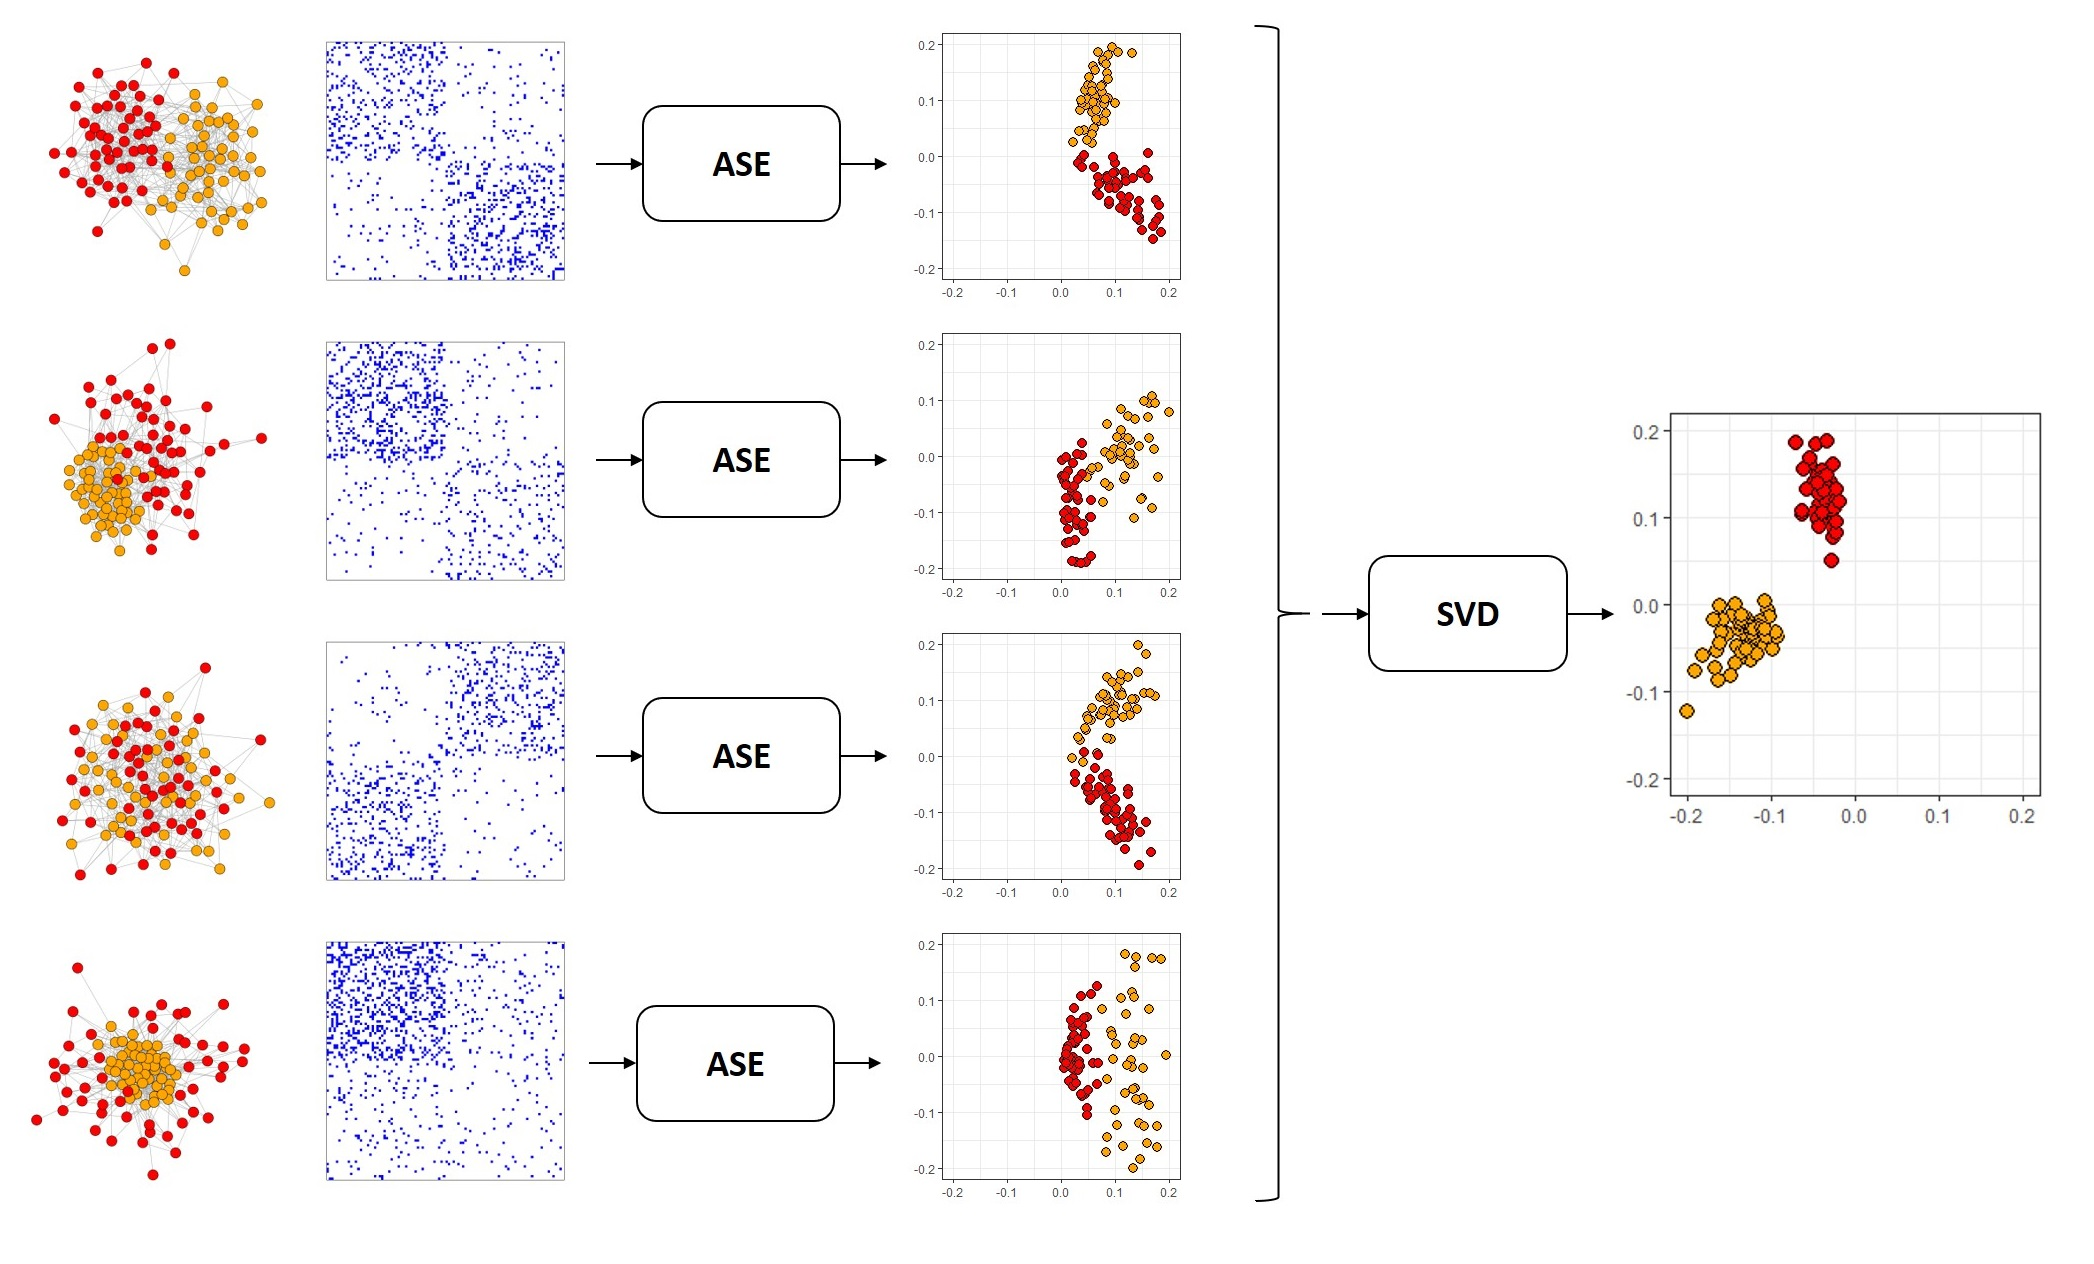
\includegraphics[width=\textwidth]{Images/mase1}
			}
			
		}
		\end{Section}
		\begin{Section}{Theoretical properties}{
				\textbf{Consistency of common subspace estimator}
				\begin{itemize}
					\item Under mild assumptions on the smallest eigenvalues of the score matrices and the sparsity of the graphs
					\begin{equation*}
					\e\left[\min_{\bW \in\mathcal{O}_d} \left\| \hat{\bV} - \bV\bW \right\|\right] \lesssim \sqrt{\frac{d}{mn}} + \frac{\sqrt{d}}{n}.
					\end{equation*}
					\item 
					\textbf{Asymptotic normality of the score}
				\item The entries of the estimated score matrices are asymptotically normally distributed, in particular,
				\begin{equation*}
					\frac{1}{\sigma_{ijk}}\left( \hat{\bR}^{(i)}  - \bW\bR^{(i)}_{jk}\bW^T + 	\bH\right)_{jk} \overset{d}{\rightarrow} \mathcal{N}(0,1)
				\end{equation*}
				\item The matrix $\e[\|\bH\|_F] = O(d/\sqrt{m})$
				\item Applications in hypothesis testing and eigenvalue estimation
				\end{itemize}
			}
		\end{Section}
	\end{minipage}
	\hfill
	%%%%%%%%%%%%%%%%% THIRD COLUMN %%%%%%%%%%%%%%%%%%%%%%%%%%%%%%%%%%%%%%%%%%%%%%
	\begin{minipage}[t]{0.3\textwidth}
		\begin{Section}{Brain network analysis}{
				\begin{minipage}{0.48\textwidth}
					\textbf{HNU1 data}
					\begin{itemize}
						\item 300 graphs constructed from diffusion magnetic resonance imaging (dMRI), with $n=200$ nodes
						\item 30 different healthy subjects, and 10 scans per subject
						\item \textbf{Goal:} identify differences and similarities between graphs
					\end{itemize}
				    \textbf{Dimensionality reduction}
				    \begin{itemize}
						\item The vertex embedding identified by MASE (top figure) reflects the anatomical location of the vertices in the brain.
						\item A multidimensional scaling of the distance between the score matrices (bottom right) locates graphs from the same subject closer to each other
					\end{itemize}
				\end{minipage}\hfill
				\begin{minipage}{0.48\textwidth}
					{\centering
						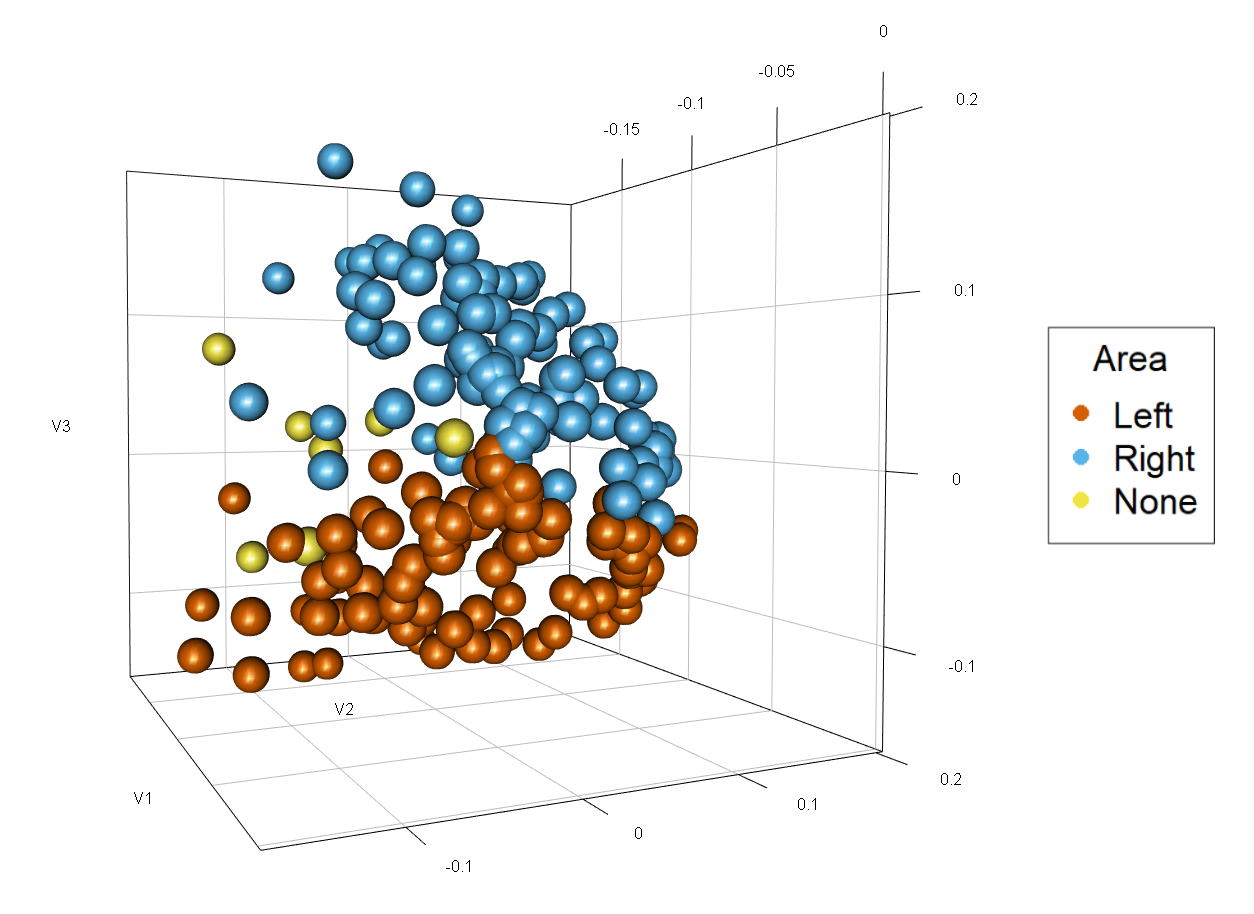
\includegraphics[width=\textwidth]{Images/HNU1-latentpositions-plot}
					}
					{\centering
						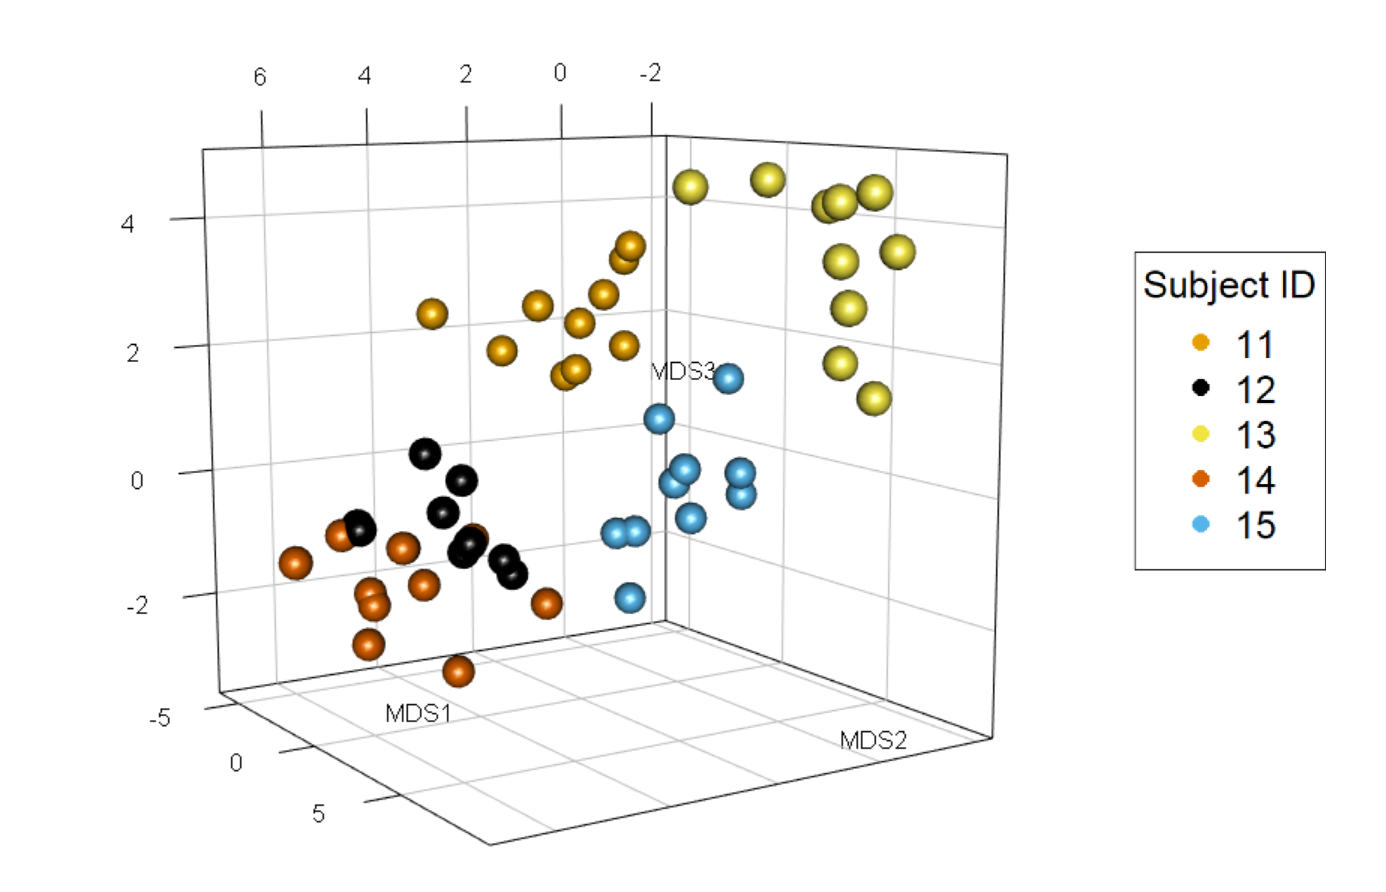
\includegraphics[width=\textwidth]{Images/HNU1-mds123-cbpalette}
					}\\					
				\end{minipage}
				

			
			\begin{minipage}{0.48\textwidth}
				\centering
				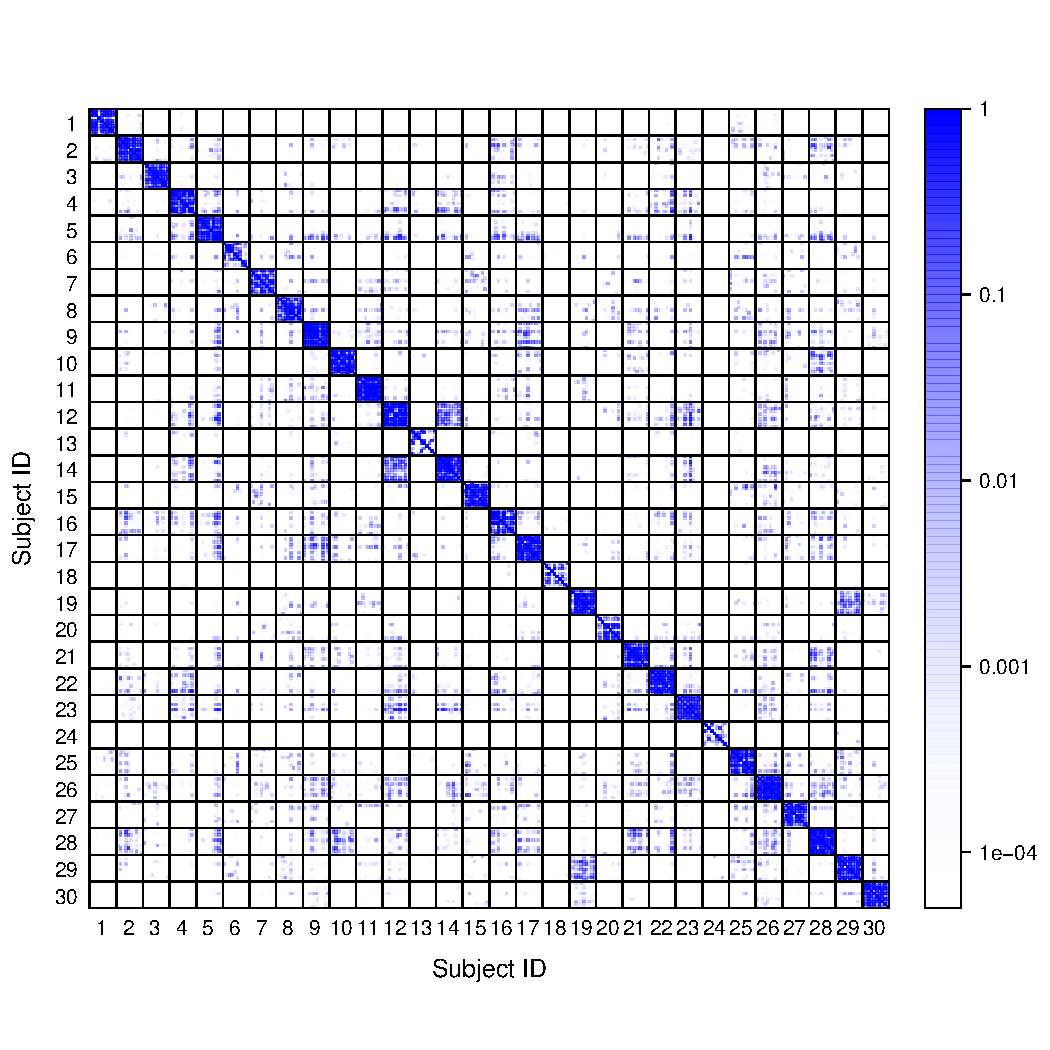
\includegraphics[width=1\textwidth]{Images/HNU1-logpvals-MASE}
			\end{minipage}
			\begin{minipage}{0.48\textwidth}
				\textbf{Graph hypothesis testing}
				\begin{itemize}
					\item For each pair of graphs $i$ and $j$, we test the hypothesis $H_0: \bR^{(i)}=\bR^{(j)}$.
					\item We use a semiparametric bootstrap approach: estimate the parameters with MASE and generate new graphs to obtain the null distribution
					\item The p-values of the test for pairs of graphs corresponding to the same subject are usually larger (diagonal blocks)
					\item COSIE can capture the similarities and differences of graphs
				\end{itemize}
			\end{minipage}
				
				
					
					\textbf{Remarks:}
					\begin{itemize}
						\item The method is computationally cheap and only involves spectral decompositions, that can be performed in parallel for each network.
						\item The dimension parameter $d$ can be estimated via the scree plot of the singular values of $\hat{\bU}$ and the eigenvalues of each $\bA^{(i)}$.
					\end{itemize}
					
					\begin{tcolorbox}[colback=blue!5,colframe=boxcol,title=Acknowledgements]
						{\footnotesize  This research has been supported by the Lifelong Learning Machines (L2M) program of the Defence Advanced
							Research Projects Agency (DARPA) via contract number HR0011-18-2-0025. This work is also supported in part
							by the D3M program of DARPA. We would like to thank Keith Levin and Elizaveta Levina for helpful discussions.
}
						
					\end{tcolorbox}	
					
					\begin{tcolorbox}[colback=blue!5,colframe=boxcol,title=References]
						\bibliographystyle{ieee} % Plain referencing style
						{\footnotesize  \bibliography{Biblio} }
						
					\end{tcolorbox}	
				}
		\end{Section}
		
		
	\end{minipage}
	\hfill
\end{minipage}

\end{document}
